\documentclass[Rapport/Rapport_main.tex]{subfiles}
\begin{document}
\subsection{Process View}
Dette view beskriver systemets dynamiske aspekter. Her angives systemprocesserne, og hvordan de kommunikerer med hinanden (med fokus på runtimeadfærd). Figur \ref{fig:capsule} illustrerer procesnedbrydningen af systemet. Her angives aspekter for programmet, som er trådkontrollet. Trådtyperne kan inddeles i tre kategorier: 
\begin{itemize}
    \item \textbf{Graphical User Interface}: Dette er GUI tråden, som render og præsenterer alle de grafiske elementer for brugeren, samt modtager og behandler inputs. Det er vigtigt at GUI-tråden ikke forstyrres fra andre operationer, fx Database Queries, således brugeroplevelse er optimal. 
    \item \textbf{Animations}: Alle animationer til den grafiske brugeroverflade udregnes og behandles på en separat tråd. Det samles med GUI-tråden til sidst og præsenteres for brugeren.
    \item \textbf{Database Queries}: Alle database queries er asynkrone og afvikles på en separat tråd. Queries bruges til at hente information, som skal præsenteres eller anvendes af GUI-tråden.
\end{itemize}
\begin{figure}[H]
    \centering
    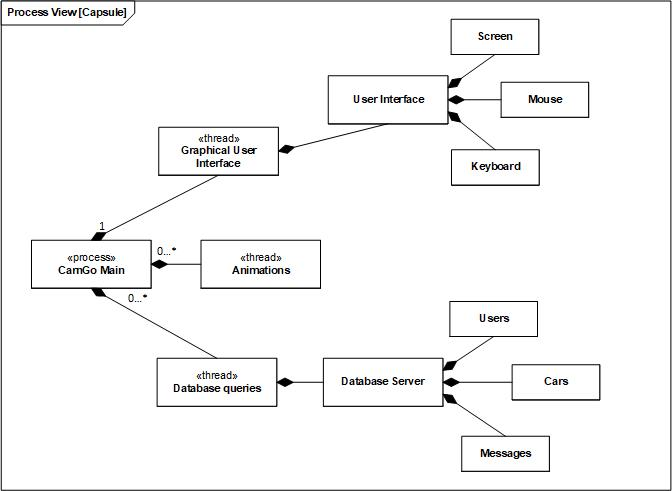
\includegraphics[width=1\textwidth]{Arkitektur/4+1View/Graphics/ProcessDiagram.jpg}
    \caption{Komponenter angives som 'kapsler'. En kapsel repræsenterer et trådkontrolleret aspekt af systemet. Der eksisterer kun en GUI-tråd, som indlæser alle grafiske elementer til brugeren. Der kan derimod opstå flere tråde for animation og queries}
    \label{fig:capsule}
\end{figure}
\noindent De abstrakte trådkontrolleret aspekter og hvordan de afvikles illustreres i et aktivitetsdiagram (Se figur \ref{fig:activity}). Her ses det hvordan at de grafiske elementer og database queries sker samtidigt. Den grafiske brugeroverflade vil løbende blive indlæst og præsenteret til brugeren. Hvis der er data fra queries, som skal præsenteres til brugeren, vil det også blive indlæst på den grafiske brugeroverflade, men det vil være uafhængigt af GUI-tråden.
\begin{figure}[H]
    \centering
    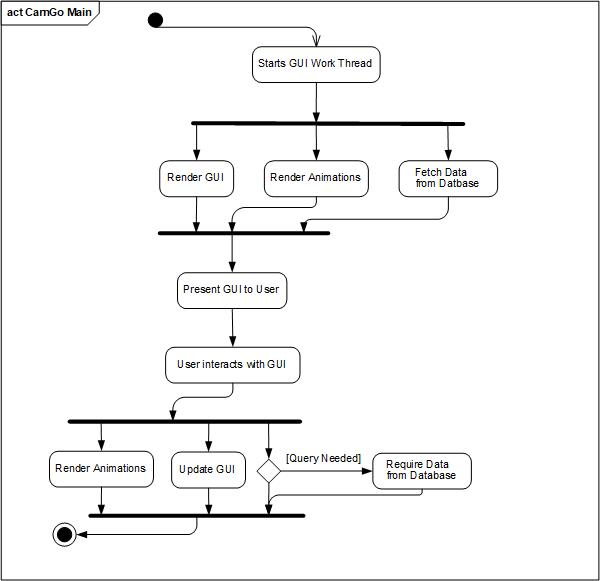
\includegraphics[width=1\textwidth]{Arkitektur/4+1View/Graphics/ActivityDiagram_Process.jpg}
    \caption{Aktivitetsdiagram for hovedprocessen for CarnGo}
    \label{fig:activity}
\end{figure}
\end{document}